\chapter{Experimental Approaches}
\label{modern_experiments}

\begin{table}[h]
    \resizebox{\textwidth}{!}{
        \begin{tabular}{ c c c c c }
            Year & Team & Approach & Upper Limit (\textit{e} cm) & Reference \\ 
            \hline
            1958 & Salpeter & Hydrogen Energy Level Splitting & $10^{-13}$ & \cite{Salpeter_1958} \\
            1958 & Feinberg & Hydrogen Energy Level Splitting & $10^{-13}$ & \cite{Feinberg_1958} \\
            1959 & Nelson et al. & Spin Precession in a Magnetic Field & $10^{-13}$ & \cite{Nelson_1959} \\
            1963 & Goldemberg, Torizuka & Scattering & $10^{-15}$ & \cite{Goldemberg_1963} \\
            1963 & Royce, Bloembergen & Paramagnetic Resonance & $1.4 \times 10^{-15}$ & \cite{Royce_Bloembergen_1963} \\
            1964 & Sandars, Lipworth & Atomic Beam & $2 \times 10^{-21}$ & \cite{Sandars_Lipworth_1964} \\
            1968 & Weisskopf et al. & Atomic Beam & $3 \times 10^{-24}$ & \cite{Weisskopf_1968} \\
            1970 & Player, Sanders & Atomic Beam & $7 \times 10^{-25}$ & \cite{Player_1970} \\
            1989 & Cho et al. & Atomic Beam & $1.4 \times 10^{-25}$ & \cite{Cho_1989} \\
            1989 & Murthy et al. & Atomic Beam & $1.5 \times 10^{-26}$ & \cite{Murthy_1989} \\
            1990 & Abdullah et al. & Atomic Beam & $2.7 \times 10^{-27}$ & \cite{Abdullah_1990} \\
            2002 & Regan et al. & Atomic Beam & $1.6 \times 10^{-27}$ & \cite{Regan_2002} \\
            2011 & Hudson et al. & Molecular Beam & $1.1 \times 10^{-27}$ & \cite{Hudson_2011} \\
            2014 & ACME & Molecular Beam & $8.7 \times 10^{-29}$ & \cite{ACME_2014} \\
            2018 & ACME & Molecular Beam & $1.1 \times 10^{-29}$ & \cite{ACME_2018} \\
        \end{tabular}
    }
    \caption{\label{tab:upper_bound_timeline} Timeline of the historical the measured upper bounds of the electron's EDM. Since around the 1970s the convention for determining an experimental upper bound has been from the largest possible eEDM that would be viable given a 90\% confidence interval on the measured non-zero value.}
\end{table}

From table \ref{tab:upper_bound_timeline} it can be seen that from 1964 to 2011 leading experiments have used atomic beams to determine an upper bound on the electron's EDM. These atomic beam experiments attempt to observe an electron's EDM by evolving a carefully selected state (using the techniques outlined in sections \ref{atomic_energy_structure}, \ref{optical_pumping} and \ref{pi_pulses}). To increase the precision of the measurement the effect is magnified through a large enhancement factor, a concept introduced in section \ref{enhancement_factor_section}.

Since 2011 molecular beams have been utilised to further decrease the upper-bound by several orders of magnitude. This improved experimental precision lies predominantly in the the greater enhancement factors of molecules such as ThO and YbF.

In this section the principles of atomic beam experiments will be covered, as well as a subsequent discussion of the more recent molecular beam experiments. Finally there will be a brief introduction to the proposed future experiments, believed to provide even greater precision.

\section{Shot-Noise Limit}
\label{general_precision_considerations}

Modern eEDM experiments have typically sought to take a measurement from the energy shift of a molecule due to eEDM interactions. Before exploring the specific approaches of these measurements, it is worth defining the shot-noise limit of a possible eEDM measurement.

We start by defining the EDM induced energy splitting between two states with an opposite parity, 

\begin{equation} \label{edm_anglular_frequency_splitting}
    \hbar \omega_{EDM} = 2 d_e E_{eff}
\end{equation}

where the energy is in the form of an angular frequency. The statistical uncertainty in $\omega_{EDM}$ for $N$ independent measurements obeying Poisson statistics is given by

\begin{equation} \label{edm_SNR}
    T \delta \omega_{EDM} = \frac{1}{\sqrt{N}}
\end{equation}

where $T$ is the interaction duration, for a more detailed explanation please refer to \cite{Vutha_2010}.

By combining equations \ref{edm_anglular_frequency_splitting} and \ref{edm_SNR} we can find the shot-noise limit of the uncertainty in the measured eEDM

\begin{equation}
    \label{shot_noise_limit}
    \delta d_e = \frac{\hbar}{2 E_{eff} T \sqrt{N}}.
\end{equation}

From this relation we can see that as a general heuristic longer interaction times, greater effective electric fields and larger ensembles of measurements will result in greater precision on the final measurement. Using this general heuristic, the atomic and molecular beam experiments discussed in this review are compared in table \ref{tab:experiment_heuristic_comparison}.

\begin{table}[h]
    \resizebox{\textwidth}{!}{
        \begin{tabular}{ c c c c c c c }
            Experiment & $E_{eff}$ (V/cm) & Coherence Time (s) & Population & Shot-noise $\delta d_e$ (e cm $\sqrt{day}$) & Section & Reference \\
            \hline
            Tl Beam & $7 \times 10^{7}$ & $2.4 \times 10^{-3}$ & $10^{9}$ & $2.1 \times 10^{-28}$ & \ref{atomic_beams} & \cite{Regan_2002} \\
            YbF Beam & $1.3 \times 10^{10}$ & $10^{-3}$ & $5 \times 10^{4}$ & $3.8 \times 10^{-28}$ & \ref{YbF_experiment} & \cite{Hudson_2011} \\
            ThO Beam & $7.8 \times 10^{10}$ & $10^{-3}$ & $10^{5}$ & $4.5 \times 10^{-29}$ & \ref{ThO_Experiment} & \cite{ACME_2018} \\
        \end{tabular}
    }
    \caption{\label{tab:experiment_heuristic_comparison} Comparison of the shot-noise limit for the discussed experiments.}
\end{table}

\section{Atomic Beam Experiments} \label{atomic_beams}

In this section we will focus on the atomic beam experiment performed by Regan et al \cite{Regan_2002}. This experiment is a useful reference as it employed many critical techniques for improving the sensitivity of the experiment, enabling it to achieve the most precise measurement with an atomic beam.

\subsection{Simplified Experiment}

\begin{figure}[h]
    \centerline{
        \resizebox{15cm}{!}{
            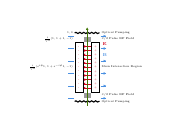
\begin{tikzpicture}[x=0.75pt,y=0.75pt]
                \definecolor{laser}{RGB}{65,117,5}
                \definecolor{electric}{RGB}{208,2,27}
                \definecolor{magnetic}{RGB}{74,144,226}
                \definecolor{rf_boxes}{RGB}{155,155,155}
                
                % Electric field arrows
                \foreach \x in {0,...,10}{
                    % Left field
                    \draw [electric, line width=0.05mm]   (2,10 - 2 * \x) -- (-2,10 - 2 * \x);
                    \draw [electric, fill=electric, line width=0.02mm] (-2,10 - 2 * \x) -- (-1,9.5 - 2 * \x) -- (-1,10.5 - 2 * \x) -- cycle;
                    
                    % Text Node
                    \draw (4,10 - 2 * \x) node [color=electric, opacity=1, align=center, scale=0.2] {\fontsize{0.01}{0}\selectfont+};
                    \draw (-4,10 - 2 * \x) node [color=electric, opacity=1, align=center, scale=0.2] {\fontsize{0.01}{0}\selectfont-};
                }
                
                % Magnetic field arrows
                \foreach \x in {0,...,5}{
                    % Left field
                    \draw [magnetic, line width=0.05mm]   (-6.5,15 - 6 * \x) -- (-9,15 - 6 * \x);

                    % Right field
                    \draw [magnetic, line width=0.05mm]   (6.5,15 - 6 * \x) -- (9,15 - 6 * \x);
                    \draw [magnetic, fill=magnetic, line width=0.02mm] (9,15 - 6 * \x) -- (8,14.5 - 6 * \x) -- (8,15.5 - 6 * \x) -- cycle;
                }
                
                % Optical Pumping Lasers
                \foreach \x in {-1,1}{
                    \draw [-, decorate, decoration={snake, amplitude=0.08mm, segment length=0.5mm, post length=0mm}] (-6, \x * 16.5) -- (6, \x * 16.5);
                    \draw (6, \x * 16.5) node [anchor=west, color=black, opacity=1, align=center, scale=0.2] {\fontsize{0.01}{0}\selectfont Optical Pumping};
                }

                % Charge Boxes
                \foreach \x in {-1,1}{
                    \draw [black, line width=0.05mm] (\x * 6,12) -- (\x * 2,12) -- (\x * 2,-12) -- (\x * 6,-12) -- cycle;
                }
                
                % laser arrow
                \draw [laser, line width=0.1mm] (0,-18.5) -- (0,18.5);
                \draw [laser, fill=laser, line width=0.02mm] (-0.5,18) -- (0,19) -- (0.5,18) -- cycle;
                
                
                \foreach \x in {-1,1}{
                    \draw (6, \x * 13.5) node [anchor=west, color=black, opacity=1, align=center, scale=0.2] {\fontsize{0.01}{0}\selectfont $\pi/2$ Pulse RF Field};
                    \foreach \y in {-1,1}{
                        % Lower RF Fields
                        \draw [rf_boxes, fill=rf_boxes, line width=0.02mm] (\x * 1.5, \y * 12.5) -- (\x * 1.5, \y * 14.5) -- (\x * 0.5, \y * 14.5) -- (\x * 0.5, \y * 12.5) -- cycle;
                    }
                }
                
                \draw (6,11) node [anchor=west, color=electric, opacity=1, align=center, scale=0.3] {\fontsize{0.01}{0}\selectfont\bf{E}};
                \draw (6,6) node [anchor=west, color=magnetic, opacity=1, align=center, scale=0.3] {\fontsize{0.01}{0}\selectfont\bf{B}};

                \draw (6, 0) node [anchor=west, color=black, opacity=1, align=center, scale=0.2] {\fontsize{0.01}{0}\selectfont Main Interaction Region};
                
                % Pumped State
                \draw (-6, 16.5) node [anchor=east, color=black, opacity=1, align=center, scale=0.2] {\fontsize{0.01}{0}\selectfont $\ket{1,0}$};
                
                % Pulsed State
                \draw (-6, 13.5) node [anchor=east, color=black, opacity=1, align=center, scale=0.2] {\fontsize{0.01}{0}\selectfont $\frac{i}{\sqrt{2}} ( \ket{1,1} + \ket{1,-1} )$};
                
                \draw (-6, 0) node [anchor=east, color=black, opacity=1, align=center, scale=0.2] {\fontsize{0.01}{0}\selectfont $\frac{i}{\sqrt{2}} ( e^{i \phi}\ket{1,1} + e^{-i \phi}\ket{1,-1} )$};
                
            \end{tikzpicture}
        }
    }
    \caption{Simplified Experimental procedure of the Thallium beam experiment \cite{Regan_2002}}
    \label{fig:simplified_atomic_beam_procedure}
\end{figure}

In figure \ref{fig:simplified_atomic_beam_procedure} a simplified experimental structure is shown. Mathematically this structure can be understood as the propagator

\begin{equation} \label{experiment_propagator}
    U_{experiment} = U_{pump} U_{\pi/2 + \alpha} U_{int} U_{\pi/2} U_{pump}.
\end{equation}

The experiment begins with a region of optical pumping achieved by a laser tuned to 378nm, which excited the $6^2P_{1/2} \rightarrow 6^2S_{1/2}$ transition. As discussed in section \ref{optical_pumping}, the probability of excitations can be calculated from the product of the Clebsch-Gordon coefficient and the hyperfine level coupling, as given in equation \ref{transition_probability}. The Clebsch-Gordon coefficients are only non-zero for excitations from the $m_F = \pm 1$ states, as shown by solid lines in figure \ref{fig:optical_pumping_scheme}. The decays from these excitations will fall with varying probabilities to the sublevels of the $6^2P_{1/2}$ and $6^2P_{3/2}$ states. It can be found that with a sufficient number of cycles the $\ket{F=1,m_F=0}$ sublevel can achieve a population of 34\% of the initial flux of atoms, with the remainder of atoms lying in the $6^2P_{3/2}$ or $\ket{F=0,m_F=0}$ dark states \cite{Regan_2001}.

Ignoring the dark states we can now consider the wavefunction of the Thallium atoms as

\begin{equation} \label{pumped_wavefunction}
    \ket{\psi} = \ket{1, 0}
\end{equation}

where our state follows the notation $\ket{F,m_F}$.

The second stage of the experiment was the application of an RF magnetic field, tuned to apply a $\pi/2$ pulse, transforming the Thallium atomic states into a superposition of $m_F = \pm 1$ states. An overview of this process is given in section \ref{pi_pulses} and the motivation for this stage is to prepare the atoms to evolve distinctly in the following main interaction region. The propagator for this process can be written as

\begin{equation} \label{proagated_pumped_wavefunction}
    U_{\pi / 2} \ket{1,0} = \frac{i}{\sqrt{2}} (\ket{1,1} + \ket{1,-1}).
\end{equation}

Once the superposition state is achieved, the thallium atoms enter the main interaction region, which consists of a strong electric field, as well as the background magnetic field. A simplified Hamiltonian, including only dipole interactions, for the atomic states in this region is

\begin{equation} \label{main_interaction_hamiltonian}
    H = - \boldsymbol{\mu} \cdot \mathbf{B} - \mathbf{d}_e \cdot \mathbf{E}_{eff}.
\end{equation}

The full picture is complicated by higher order features, a discussion of the complete Hamiltonian can be found in \cite{Regan_2001, Regan_2002}. By applying the corresponding propagator for time T the initial superposition state will become

\begin{equation} \label{main_interaction_propagated_state}
    \frac{i}{\sqrt{2}} U_{int} (\ket{1,1} + \ket{1,-1}) = \frac{i}{\sqrt{2}} (e^{i \phi} \ket{1, 1} + e^{-i \phi} \ket{1, -1})
\end{equation}

where the phase $\phi$ is given by

\begin{equation} \label{main_interaction_propagated_phase}
    \phi = (\boldsymbol{\mu} \cdot \mathbf{B} + \mathbf{d}_e \cdot \mathbf{E}_{eff}) \frac{T}{\hbar}.
\end{equation}

This phase can be visualised as a rotation in the x-y plane of the Bloch sphere, as shown in figure \ref{fig:bloch_sphere}. 

\begin{figure}[h]
    \centerline{
        \resizebox{12cm}{!}{
            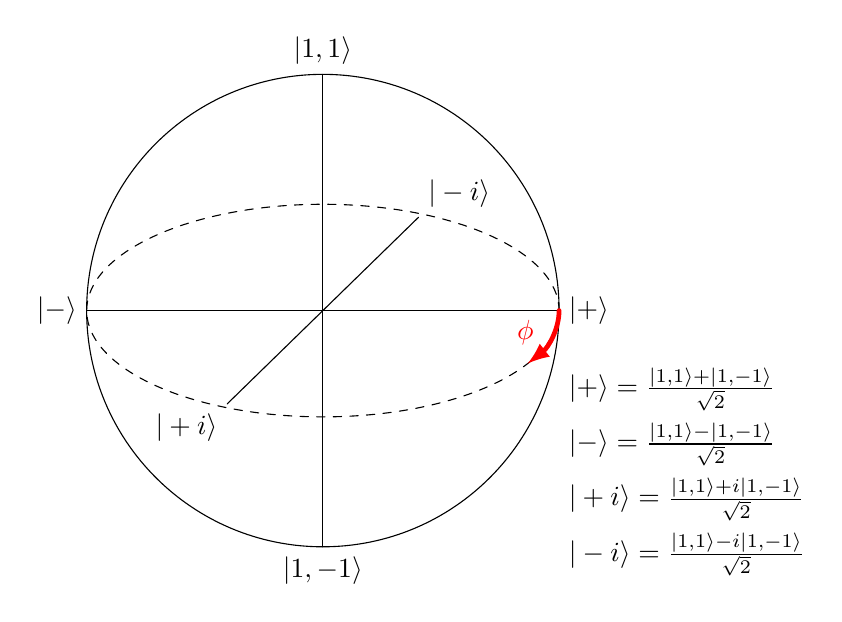
\begin{tikzpicture}[line cap=round, line join=round]
              \draw(0,0) circle (3cm);
              \draw [rotate around={0.:(0.,0.)},dash pattern=on 3pt off 3pt] (0,0) ellipse (3cm and 1.35cm);

              \draw (0,-3) -- (0,3);
              \draw (-3,0) -- (3,0);
              \draw (-1.215,-1.185) -- (1.215,1.185);
              
              \draw (-1.215,-1.185) node[anchor=north east] {$|+i\rangle$};
              \draw (1.215,1.185) node[anchor=south west] {$|-i\rangle$};
              
              \draw (3,0) node[anchor=west] {$|+\rangle$};
              \draw (-3,0) node[anchor=east] {$|-\rangle$};
              
              \draw (0,3) node[anchor=south] {$|1,1\rangle$};
              \draw (0,-3) node[anchor=north] {$|1,-1\rangle$};
              
              \draw (3,-1) node[anchor=west] {$|+\rangle = \frac{|1,1\rangle + |1,-1\rangle}{\sqrt{2}}$};
              \draw (3,-1.7) node[anchor=west] {$|-\rangle = \frac{|1,1\rangle - |1,-1\rangle}{\sqrt{2}}$};
              \draw (3,-2.4) node[anchor=west] {$|+i\rangle = \frac{|1,1\rangle + i |1,-1\rangle}{\sqrt{2}}$};
              \draw (3,-3.1) node[anchor=west] {$|-i\rangle = \frac{|1,1\rangle - i |1,-1\rangle}{\sqrt{2}}$};
              
              \draw [red, line width=0.6mm, -latex] (0:3cm and 1.35cm) arc (0:-30:3cm and 1.35cm);
              \draw (2.8,0) node[red, anchor=north east] {$\phi$};
            %   \draw[thick, red, -latex] ($(0, 0) + (30:3cm and 2cm)$(P) arc (30:150:3cm and 2cm)
            \end{tikzpicture}
        }
    }
    \caption{Bloch sphere representation for the two level system}
    \label{fig:bloch_sphere}
\end{figure}

After the main interaction region, the Thallium atoms enter another magnetic RF field which applies a $\pi/2$, however in this case there is an additional offset phase, $\alpha$. The additional phase $\alpha$ will be key to determining the EDM measurement from the signal collected in the subsequent stage. The RF field transforms the thallium atoms with the following propagator

\begin{equation}
	U_{\frac{\pi}{2} + \alpha} = \begin{pmatrix}
		-e^{\frac{i}{2}(\alpha + \frac{\pi}{2})} \sin(\alpha) & -e^{\frac{i}{2}(\alpha + \frac{\pi}{2})} \cos(\alpha) & 0 \\
	    -\frac{e^{-\frac{i}{2}(\alpha + \frac{\pi}{2})} \cos(\alpha)}{\sqrt{2}} & -\frac{e^{-\frac{i}{2}(\alpha + \frac{\pi}{2})} \sin(\alpha)}{\sqrt{2}} & \frac{e^{-\frac{i}{2}(\alpha + \frac{\pi}{2})}}{\sqrt{2}} \\
	    -\frac{e^{-\frac{i}{2}(\alpha + \frac{\pi}{2})} \cos(\alpha)}{\sqrt{2}} & -\frac{e^{-\frac{i}{2}(\alpha + \frac{\pi}{2})} \sin(\alpha)}{\sqrt{2}} & -\frac{e^{-\frac{i}{2}(\alpha + \frac{\pi}{2})}}{\sqrt{2}} \\
	\end{pmatrix}
\end{equation}

written in the $\{|1, 0 \rangle, |1, 1 \rangle, |1, -1 \rangle\}$ basis. By applying this propagator and then taking the modulus squared we find  the probabilities of states $\ket{1, 1}$ and $\ket{1, -1}$ to be

\begin{equation} \label{final_state_probabilities}
        P_{\ket{1, 1}} = P_{\ket{1, -1}} = \cos^2(\phi) \sin^2(\alpha) + \sin^2(\phi).
\end{equation}

\begin{figure}[h]
    \centering
    \includegraphics[width=150mm,scale=0.5]{images/prob_thallium_atoms.png}
    \caption{Probability of thallium atoms occupying states $\ket{1, \pm 1}$}
    \label{fig:thallium_probability}
\end{figure}

This probability is visualised in figure \ref{fig:thallium_probability}. The form of the atomic hyperfine state probability function is key to the final stage of the experiment, which seeks to extract a signal for the phase $\phi$. This signal is captured from the fluorescence of decays induced by another region of optical pumping, which follows the same pumping scheme previously discussed and visualised in figure \ref{fig:optical_pumping_scheme}. The measured count of decays corresponds to the number of excitations, which is dependent on the number of Thallium atoms lying in the $m_F = \pm 1$ states. Therefore by capturing a count of the decays for a range of $\alpha$ configurations, the experimenters were able to determine a measure of $\frac{d P_{\ket{1, \pm 1}}}{d\alpha}$, which from figure \ref{fig:thallium_probability} can be seen to be proportional to $\phi$. By conducting the experiment with the electric field both parallel and anti-parallel to the magnetic field, the experimenters were able to isolate the evolution corresponding to the eEDM interaction.

\subsection{Complete Experiment}

\begin{figure}[h]
    \centerline{
        \resizebox{10cm}{!}{
            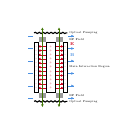
\begin{tikzpicture}[x=0.75pt,y=0.75pt]
                \definecolor{laser}{RGB}{65,117,5}
                \definecolor{electric}{RGB}{208,2,27}
                \definecolor{magnetic}{RGB}{74,144,226}
                \definecolor{rf_boxes}{RGB}{155,155,155}
                
                % Electric field arrows
                \foreach \x in {0,...,10}{
                    % Left field
                    \draw [electric, line width=0.05mm]   (-2,10 - 2 * \x) -- (-6,10 - 2 * \x);
                    \draw [electric, fill=electric, line width=0.02mm] (-6,10 - 2 * \x) -- (-5,9.5 - 2 * \x) -- (-5,10.5 - 2 * \x) -- cycle;
                    
                    % Right field
                    \draw [electric, line width=0.05mm]   (2,10 - 2 * \x) -- (6,10 - 2 * \x);
                    \draw [electric, fill=electric, line width=0.02mm] (6,10 - 2 * \x) -- (5,9.5 - 2 * \x) -- (5,10.5 - 2 * \x) -- cycle;
                    
                    % Text Node
                    \draw (0,10 - 2 * \x) node [color=electric, opacity=1, align=center, scale=0.2] {\fontsize{0.01}{0}\selectfont+};
                    \draw (7,10 - 2 * \x) node [color=electric, opacity=1, align=center, scale=0.2] {\fontsize{0.01}{0}\selectfont-};
                    \draw (-7,10 - 2 * \x) node [color=electric, opacity=1, align=center, scale=0.2] {\fontsize{0.01}{0}\selectfont-};
                }
                
                % Magnetic field arrows
                \foreach \x in {0,...,5}{
                    % Left field
                    \draw [magnetic, line width=0.05mm]   (-8.5,15 - 6 * \x) -- (-11,15 - 6 * \x);

                    % Right field
                    \draw [magnetic, line width=0.05mm]   (8.5,15 - 6 * \x) -- (11,15 - 6 * \x);
                    \draw [magnetic, fill=magnetic, line width=0.02mm] (11,15 - 6 * \x) -- (10,14.5 - 6 * \x) -- (10,15.5 - 6 * \x) -- cycle;
                }
                
                % Optical Pumping Lasers
                \foreach \x in {-1,1}{
                    \draw [-, decorate, decoration={snake, amplitude=0.08mm, segment length=0.5mm, post length=0mm}] (-8, \x * 16.5) -- (8, \x * 16.5);
                    \draw (8, \x * 16.5) node [anchor=west, color=black, opacity=1, align=center, scale=0.2] {\fontsize{0.01}{0}\selectfont Optical Pumping};
                }

                % Charge Boxes
                \draw [black, line width=0.05mm] (-8,12) -- (-6,12) -- (-6,-12) -- (-8,-12) -- cycle;
                \draw [black, line width=0.05mm] (-2,12) -- (2,12) -- (2,-12) -- (-2,-12) -- cycle;
                \draw [black, line width=0.05mm] (8,12) -- (6,12) -- (6,-12) -- (8,-12) -- cycle;
                
                % Laser arrows
                \foreach \x in {-1,1}{
                    \draw [laser, line width=0.1mm] (\x * 4,-18.5) -- (\x *  4,18.5);
                    \foreach \y in {-1, 1} {
                        \draw [laser, fill=laser, line width=0.02mm] (\x * 4.5, \y * 18) -- (\x * 4, \y * 19) -- (\x * 3.5, \y * 18) -- cycle;
                    }
                }
                
                \foreach \x in {-1,1}{
                    \draw (8, \x * 13.5) node [anchor=west, color=black, opacity=1, align=center, scale=0.2] {\fontsize{0.01}{0}\selectfont RF Field};
                    \foreach \y in {-1,1}{
                        % Lower RF Fields
                        \draw [rf_boxes, fill=rf_boxes, line width=0.02mm] (\x * 5.5, \y * 12.5) -- (\x * 5.5, \y * 14.5) -- (\x * 4.5, \y * 14.5) -- (\x * 4.5, \y * 12.5) -- cycle;
                        \draw [rf_boxes, fill=rf_boxes, line width=0.02mm] (\x * 3.5, \y * 12.5) -- (\x * 3.5, \y * 14.5) -- (\x * 2.5, \y * 14.5) -- (\x * 2.5, \y * 12.5) -- cycle;
                    }
                }
                
                \draw (8,11) node [anchor=west, color=electric, opacity=1, align=center, scale=0.3] {\fontsize{0.01}{0}\selectfont\bf{E}};
                \draw (8,6) node [anchor=west, color=magnetic, opacity=1, align=center, scale=0.3] {\fontsize{0.01}{0}\selectfont\bf{B}};

                \draw (8, 0) node [anchor=west, color=black, opacity=1, align=left, scale=0.2] {\fontsize{0.01}{0}\selectfont Main Interaction Region};
                
            \end{tikzpicture}
        }
    }
    \caption{Experimental procedure of the Thallium beam experiment \cite{Regan_2002}}
    \label{fig:complete_atomic_beam_procedure}
\end{figure}

Whilst the simplified experiment above covers the fundamentals of the experiment, it misses several major subtleties, without which the experiment would be far less accurate. The major source of noise in the experiment is the significant impact of fluctuations in the magnetic field compared to the weak hypothesised eEDM interaction. Several strategies were employed to mitigate this impact, these strategies are be briefly outlined below.

\subsubsection{Dual Beam Electric Fields}

Instead of conducting the experiment with a single arrangement of electric and magnetic field alignment, the team used a second beam, adjacent to the first, with an opposite electric field direction. This was achieved by using a three electrode configuration, as visualised in figure \ref{fig:complete_atomic_beam_procedure}. With this configuration the experiment did not require the electric field to be reversed between runs, a process which would introduce systematic errors due to erroneous magnetic fields and other noise.

\subsubsection{Sodium Beams}

As opposed to attempting to perfectly shield the experiment, the experimenters utilised a control beam of sodium. Sodium is also a para-magnetic atom, however it has a much smaller enhancement factor. Therefore by measuring the magnetic field induced phase shift in sodium, the experimenters were able to in real time subtract the noise in the variation of the magnetic field from the measurement of the thallium phase shift.

\subsubsection{Dual Beam Directions}

Another source of anomalous magnetic field effects arose from the motion of the atoms. The atomic beams had velocities of the order $10^2$m$\text{s}^{-1}$, with significant variation in the velocity distribution. This velocity variation posed a major source of systematic error since for a charge travelling through an electric field an effective magnetic field $\mathbf{B}_{eff}$ is induced, as governed by equation \ref{induced_magnetic field}.

\begin{equation} \label{induced_magnetic field}
    \mathbf{B}_{eff} = \frac{1}{c^2}(\mathbf{v} \times \mathbf{E})
\end{equation}

By using two counter propagating beams on each channel, the experimenters were able to cancel out this induced magnetic field.

\section{Molecular Beams}

Since 2011 leading experimental bounds on the electron's EDM have utilised molecular beams of Ytterbium Fluoride (YbF) \cite{Hudson_2011} or Thorium Monoxide (ThO) \cite{ACME_2014, ACME_2018}. The idea of utilising molecular beams is not new, as early as 1967 Sandars presented the case for molecular beams, arguing that their increased polarizability would lead to much greater enhancement factors, and therefore a much more precise experiment \cite{Sandars_1967}, a qualitative discussion of the greater enhancement factor is provided in section \ref{enhancement_factor_section}. Another motivation for utilising molecular beams is their weaker sensitivity to motional magnetic fields, which were found to be a major limitation in atomic beam experiments. However, despite these benefits these molecules pose major challenges in practice, such as being highly reactive, making them hard to work with in large numbers, as well as having more complex energy level structure, due to the additional internal degrees of freedom present in a molecule relative to an atom.

\subsection{Ytterbium Fluoride Experiment} \label{YbF_experiment}

Since as early as 2002 eEDM experiments have been conducted using Ytterbium Fluoride \cite{Hudson_2002}. However it was not until 2011 that an experimental upper bound was achieved with a YbF beam. This experiment followed a similar experimental approach to the previously discussed atomic beam experiment (see section \ref{atomic_beams}) \cite{Kara_2012}. The major difference when working with a molecular beam is the vibrational and rotational degrees of freedom. These complications are removed when considering the ground state of YbF. In this state the molecule can be understood as a $\text{Yb}^2+$ core and an $F^-$ ion with an unpaired valence electron, with the valence electron behaving similarly to an alkali atom's valence electron.

The experiment begins with a regime of optical pumping equivalent to the atomic beam experiment mentioned previously. The ground state of YbF is characterised by two hyperfine level, an $F=0$ singlet state and an $F=1$ triplet state. The specific pumping scheme is shown in figure \ref{fig:YbF_optical_pumping_scheme}, and can be seen to mirror the scheme for Thallium, shown in figure \ref{fig:optical_pumping_scheme}.

\begin{figure}[h]
    \centerline{
        \resizebox{10cm}{!}{
            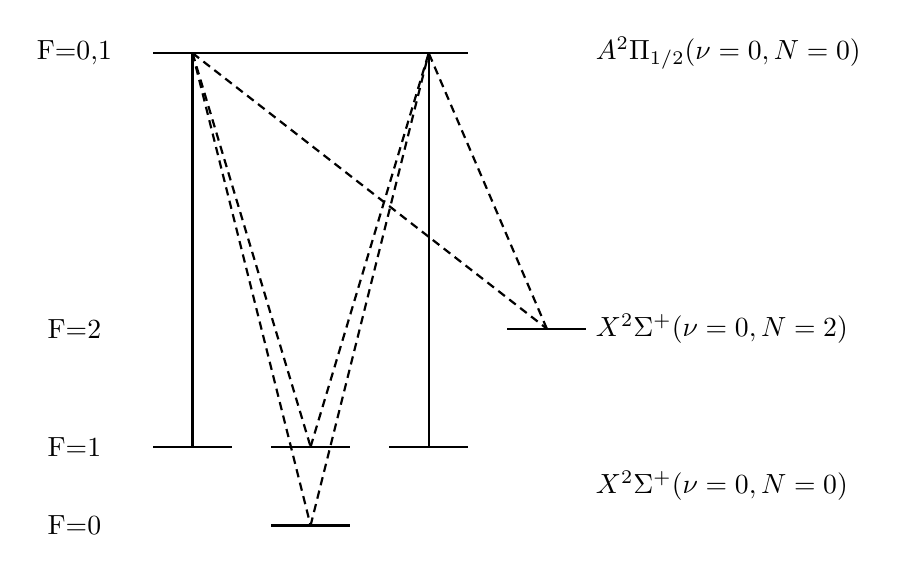
\begin{tikzpicture}[
              scale=0.5,
              level/.style={thick},
              decay/.style={thick,densely dashed},
              driven/.style={thick},
              classical/.style={thin,double,<->,shorten >=4pt,shorten <=4pt,>=stealth}
            ]
            % Level: A2Pi1/2
            \draw[level] (2cm,-2cm) -- (10cm,-2cm);
            \node at (0cm, -2cm) {F=0,1};
            
            \node[anchor=west] at (13cm, -2cm) {$A^2\Pi_{1/2} (\nu=0, N=0)$};
            
            % Level: 6P3/2
            \draw[level] (11cm,-9cm) -- (13cm,-9cm);
            \node at (0cm, -9cm) {F=2};
            \node[anchor=west] at (13cm, -9cm) {$X^2\Sigma^{+} (\nu=0, N=2)$};

            % Level: 6P1/2
            \draw[level] (2cm,-12cm) -- (4cm,-12cm);
            \draw[level] (5cm,-12cm) -- (7cm,-12cm);
            \draw[level] (8cm,-12cm) -- (10cm,-12cm);
            \node at (0cm, -12cm) {F=1};

            \draw[level] (5cm,-14cm) -- (7cm,-14cm);
            \node at (0cm, -14cm) {F=0};
            
            \node[anchor=west] at (13cm, -13cm) {$X^2\Sigma^{+} (\nu=0, N=0)$};
            
            % Driven Transitions
            \draw[driven] (3cm,-12cm) -- (3cm,-2cm);
            \draw[driven] (9cm,-12cm) -- (9cm,-2cm);
            
            % Decays
            \draw[decay] (3cm,-2cm) -- (6cm,-12cm);
            \draw[decay] (6cm,-12cm) -- (9cm,-2cm);

            \draw[decay] (3cm,-2cm) -- (6cm,-14cm);
            \draw[decay] (6cm,-14cm) -- (9cm,-2cm);

            \draw[decay] (3cm,-2cm) -- (12cm,-9cm);
            \draw[decay] (12cm,-9cm) -- (9cm,-2cm);
            
            \end{tikzpicture}
        }
    }
    \caption{Optical pumping of YbF for $m_F=0$ state selection, driven excitations are denoted by solid lines and spontaneous decays are denoted by dashed lines}
    \label{fig:YbF_optical_pumping_scheme}
\end{figure}

Unlike in the Thallium experiment, the YbF molecules then undergo a $\pi$ pulse in a subsequent RF region. However, despite the experiment using a $\pi$ instead of a $\pi/2$ pulse, the goal of the pulse was equivalent, producing a superposition state of $m_F = \pm 1$ states. The superposition state then passed through an interaction region where they evolved in an equivalent fashion to the atomic beam case, subject to both a magnetic and electric field.

After the interaction region, the pulses similarly undergo another $\pi$ pulse which transforms them to a superposition state of $F=0$ and $F=1$ states. Finally the population of molecules in the $F=0$ state is measured by laser induced fluorescence.

\paragraph{Experimental Accuracy and Limitations}

The major improvement made by the YbF experiment was the greatly reduced sensitivity to magnetic interaction noise relative to the electric dipole interaction. This reduced sensitivity resulted from the much greater effective electric fields achievable with YbF, as seen in table \ref{tab:enhancement_factors}.

A much greater relative electric field not only made the EDM interaction much greater, but it also had secondary effects which further reduced noise. Previously we discussed the application of dual beam directions in the Thallium beam experiment, so as to cancel the effective magnetic fields induced by the velocities of the atoms. It turns out that this effect is inherently reduced for the YbF experiment. Due to the increased polarisability of the molecule, and therefore its much greater alignment to the electric field direction (which is parallel to the magnetic field), the motional magnetic field effects, which arises from a magnetic field perpendicular to the electric field are greatly suppressed. This systematic effect was the major limiting factor of previous EDM experiments, hence this development explains much of the improved sensitivity, an improvement not apparent in the simple shot-noise limits in table \ref{tab:experiment_heuristic_comparison}.

\subsection{Thorium Monoxide Experiment}
\label{ThO_Experiment}

Molecular beam searches for a non-zero eEDM have not been restricted to YbF, instead many other molecules have been explored, notably in early experiments using lead oxide (PbO) and more recent experiments using thorium monoxide (ThO). These experiments were motivated by the convenient $\Omega$-doublet states found in both molecules, which would allow for greater sensitivity and reduction of systematic effects.

\begin{figure}[h]
    \centerline{
        \resizebox{14cm}{!}{
            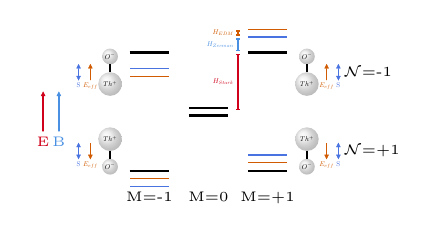
\begin{tikzpicture}[
              scale=0.5,
              level/.style={thick},
              decay/.style={thick,densely dashed},
              driven/.style={thick},
              classical/.style={thin,double,<->,shorten >=4pt,shorten <=4pt,>=stealth}
            ]
            \definecolor{electric}{RGB}{208,2,27}
            \definecolor{electric_eff}{RGB}{208, 91, 2}
            \definecolor{magnetic}{RGB}{74,144,226}
            \definecolor{spin}{RGB}{74, 115, 226}
            
            \foreach \x in {-1, 1}{
                \foreach \y in {-1, 1}{
                    % ThO Molecule
                    \shade[ball color=gray!40, opacity=0.4] (\x * 2.5cm, \y * 0.7cm) circle (0.3cm);
                    \node[scale=0.25] at (\x * 2.5cm, \y * 0.7cm) {$Th^{+}$};
                    \shade[ball color=gray!40, opacity=0.4] (\x * 2.5cm, \y * 1.4cm) circle (0.2cm);
                    \node[scale=0.25] at (\x * 2.5cm, \y * 1.4cm) {$O^{-}$};
                    \draw[level] (\x * 2.5cm, \y * 1.2cm) -- (\x * 2.5cm, \y * 1cm);

                    % Electric Field Direction
                    \draw [electric_eff, fill=electric_eff, line width=0.05mm] (\x * 3cm, \y * 1.2cm) -- (\x * 2.95cm, \y * 1.1cm) -- (\x * 3.05cm, \y * 1.1cm) -- cycle;
                    \draw [electric_eff, fill=electric_eff, line width=0.1mm] (\x * 3cm, \y * 1.1cm) -- (\x * 3cm, \y * 0.8cm) -- cycle;
                    \node[electric_eff, scale=0.25, anchor=north] at (\x * 3cm, {(\y * 1cm) - 0.2cm}) {$E_{eff}$};

                    % Spin
                    \draw [spin, fill=spin, line width=0.1mm] (\x * 3.3cm, \y * 1.1cm) -- (\x * 3.3cm, \y * 0.8cm) -- cycle;
                    \ifthenelse{\equal{\x}{1}}{
                        \draw [spin, fill=spin, line width=0.05mm] (\x * 3.3cm, {(\y * 1cm) - 0.2cm}) -- (\x * 3.25cm, {(\y * 1cm) - 0.1cm}) -- (\x * 3.35cm, {(\y * 1cm) - 0.1cm}) -- cycle;
                    }{
                        \draw [spin, fill=spin, line width=0.05mm] (\x * 3.3cm, {(\y * 1cm) + 0.2cm}) -- (\x * 3.25cm, {(\y * 1cm) + 0.1cm}) -- (\x * 3.35cm, {(\y * 1cm) + 0.1cm}) -- cycle;
                    }
                    \node[spin, scale=0.25, anchor=north] at (\x * 3.3cm, {(\y * 1cm) - 0.2cm}) {S};
                }
            }

            % M = 1
            \draw[level] (1cm,1.5cm) -- (2cm,1.5cm);
            \draw[level] (1cm,-1.5cm) -- (2cm,-1.5cm);
            \node[anchor=north, font=\tiny] at (1.5cm, -1.8cm) {M=+1};
            
            % M = 1, N = +1
            \draw[level, color=spin, line width=0.2mm] (1cm,1.9cm) -- (2cm,1.9cm);
            \draw[level, color=electric_eff, line width=0.1mm] (1cm,2.1cm) -- (2cm,2.1cm);
            
            % Stark Shift
            \draw[level, color=electric, line width=0.2mm] (0.75cm,0.05cm) -- (0.75cm,1.45cm);
            \draw[level, color=electric, line width=0.2mm] (0.7cm,0.05cm) -- (0.8cm,0.05cm);
            \draw[level, color=electric, line width=0.2mm] (0.7cm,1.45cm) -- (0.8cm,1.45cm);
            \node[electric, anchor=east, scale=0.25] at (0.7cm, 0.75cm) {$H_{Stark}$};
            
            % Zeeman Shift
            \draw[level, color=magnetic, line width=0.2mm] (0.75cm,1.55cm) -- (0.75cm,1.85cm);
            \draw[level, color=magnetic, line width=0.2mm] (0.7cm,1.55cm) -- (0.8cm,1.55cm);
            \draw[level, color=magnetic, line width=0.2mm] (0.7cm,1.85cm) -- (0.8cm,1.85cm);
            \node[magnetic, anchor=east, scale=0.25] at (0.7cm, 1.7cm) {$H_{Zeeman}$};
            
            % EDM Shift
            \draw[level, color=electric_eff, line width=0.2mm] (0.75cm,1.95cm) -- (0.75cm,2.05cm);
            \draw[level, color=electric_eff, line width=0.2mm] (0.7cm,1.95cm) -- (0.8cm,1.95cm);
            \draw[level, color=electric_eff, line width=0.2mm] (0.7cm,2.05cm) -- (0.8cm,2.05cm);
            \node[electric_eff, anchor=east, scale=0.25] at (0.7cm, 2cm) {$H_{EDM}$};
            
            % M = 1, N = -1
            \draw[level, color=spin, line width=0.2mm] (1cm,-1.1cm) -- (2cm,-1.1cm);
            \draw[level, color=electric_eff, line width=0.1mm] (1cm,-1.3cm) -- (2cm,-1.3cm);

            % M = 0
            \draw[level] (-0.5cm,0.1cm) -- (0.5cm,0.1cm);
            \draw[level] (-0.5cm,-0.1cm) -- (0.5cm,-0.1cm);
            \node[anchor=north, font=\tiny] at (0cm, -1.8cm) {M=0};

            % M = -1
            \draw[level] (-2cm,1.5cm) -- (-1cm,1.5cm);
            \draw[level] (-2cm,-1.5cm) -- (-1cm,-1.5cm);
            \node[anchor=north, font=\tiny] at (-1.5cm, -1.8cm) {M=-1};
            
            % M = -1, N = +1
            \draw[level, color=spin, line width=0.2mm] (-1cm,1.1cm) -- (-2cm,1.1cm);
            \draw[level, color=electric_eff, line width=0.1mm] (-1cm,0.9cm) -- (-2cm,0.9cm);
            
            % M = -1, N = -1
            \draw[level, color=spin, line width=0.2mm] (-1cm,-1.9cm) -- (-2cm,-1.9cm);
            \draw[level, color=electric_eff, line width=0.1mm] (-1cm,-1.7cm) -- (-2cm,-1.7cm);
            
            % Magnetic Field
            \draw [magnetic, fill=magnetic, line width=0.05mm] (-3.8cm, 0.5cm) -- (-3.85cm, 0.4cm) -- (-3.75cm, 0.4cm) -- cycle;
            \draw [magnetic, fill=magnetic, line width=0.2mm] (-3.8cm, -0.5cm) -- (-3.8cm, 0.4cm) -- cycle;
            \node[anchor=north, color=magnetic, font=\tiny] at (-3.8cm, -0.4cm) {B};
            
            % Electric Field
            \draw [electric, fill=electric, line width=0.05mm] (-4.2cm, 0.5cm) -- (-4.25cm, 0.4cm) -- (-4.15cm, 0.4cm) -- cycle;
            \draw [electric, fill=electric, line width=0.2mm] (-4.2cm, -0.5cm) -- (-4.2cm, 0.4cm) -- cycle;
            \node[anchor=north, color=electric, font=\tiny] at (-4.2cm, -0.4cm) {E};
            
            \node[anchor=west, font=\tiny] at (3.2cm, 1cm) {$\mathcal{N}$=-1};
            \node[anchor=west, font=\tiny] at (3.2cm, -1cm) {$\mathcal{N}$=+1};
            
            \end{tikzpicture}
        }
    }
    \caption{An energy level diagram for the ThO H state in external magnetic and electric fields, showing an example of $\Omega$ doublets. The molecule undergoes Stark, Zeeman and EDM interaction energy shifts, where the relative signs of the energy shifts are given by: sign($H_{Stark}$) = M, sign($H_{Zeeman}$) = -$\mathcal{N}$ and sign($H_{EDM}$) = -$M \mathcal{N}$. It can be seen that the relative signs of the EDM and Zeeman interactions can be reversed by only considering specific polarisation states, without any need to change the applied fields.}
    \label{fig:ThO_energy_levels}
\end{figure}

Before discussing the individual experiments, it is worth providing a brief overview of $\Omega$-doublets and their application in eEDM experiments. $\Omega$-doublets are closely spaced states of opposite polarisation parity, this means that the internal electric field of these states are defined by the parity of the state. A detailed discussion of these states can be found in \cite{Vutha_2010}, however for this discussion the key properties to note are the:

\begin{description}
    \item[Field Independent eEDM Shift Reversal] Depending on the orientation of the polar molecule with respect to parallel electric and magnetic fields the relative direction of the Zeeman and EDM energy shifts will differ, as seen in figure \ref{fig:ThO_energy_levels}. This allows the Zeeman energy shift to be cancelled by subtracting the quantum beat frequencies of the two orientations. Quantum beats are the decay fluorescence interference patterns resulting from a superposition of non-zero spin projection states ($m \neq 0$) decaying onto an $m=0$ state and interfering with each other due to a phase difference. In practice this process is more complex as one has to account for the Stark shift, a more detailed discussion of this effect can be found in \cite{Hamilton_2010}. In figure \ref{fig:comagnetometer_in_action} an example of this application of $\Omega$-doublets can be seen.
    
    \item[Greater Enhancement Factor] $\Omega$-doublets also contribute to the previously mentioned large enhancement factor which allows the experiment to be performed with a modest electric field. By not needing to maximise the electric field many systematic effects associated with this field and the correlated magnetic fields produced by leakage currents can be avoided.
\end{description}

\begin{figure}[h]
    \centering
    \includegraphics[width=120mm,scale=0.5]{images/magnetometer.PNG}
    \caption{An example of the application of an $\Omega$-doublet in the cancelling of magnetic field fluctuation. Below the individual state florescence signals are shown and on top the florescence signals are subtracted, figure reproduced from \cite{Hamilton_2010}.}
    \label{fig:comagnetometer_in_action}
\end{figure}

In 2001 DeMille et al first proposed using PbO, the motivation for its use was the possibility of conducting the experiment in a vapor cell, allowing for much higher densities than in the traditional beam approach, as well as the discussed reduction in systematic effects through use of $\Omega$-doublet field reversal \cite{DeMille_2001}. However, despite these advantages, in practice complications arising from electric and magnetic field gradients led to additional systematic effects, resulting in a less sensitive measurement than the previous YbF experiment \cite{Eckel_2013}.

More recently DeMille and the ACME (Advanced Cold Molecule Electron) collaboration have switched to using ThO, owing to its $\Omega$-doublet state, its greater enhancement factor, as well as other useful properties, such as its relatively stable ground state and its amenability to expansion cooling, allowing for a low velocity, high flux beam. Since 2014 the ACME collaboration has measured the leading experimental upper bounds on the eEDM. These measurements used ThO in a similar beam approach to the earlier YbF experiment (see section \ref{YbF_experiment}) and the preceding atomic beam experiments (see section \ref{atomic_beams}).

The main difference from previous experiments and the ACME 2014 measurement \cite{ACME_2014} was incorporating $\Omega$-doublet parity state selection into the optical pumping scheme. Since the $\Omega$-doublet states are split by a significant Stark shift, as indicated in figure \ref{fig:ThO_energy_levels}, the detuned $\Omega$-doublet state will be a dark state and will act as the initial state of the experiment. This experiment achieved an order of magnitude smaller upper limit on the eEDM, placing the limit at $8.7 \times 10^{-29}$ e cm.

In 2018 the ACME collaboration improved on this limit by increasing the flux of ThO molecules usable in the measurement. The previous approach of state selection via optical pumping achieved an efficiency of approximately $6\%$. Through employing a Stimulated Raman Adiabatic Passage (STIRAP) process the experiment managed to reach efficiencies of $75\% \pm 5\%$ \cite{Panda_2016}. STIRAP allows for two states of a three level system to be coupled via a third intermediate state, whilst also not populating the intermediate state. By not populating this intermediate state the process becomes more efficient as there will not be spontaneous emission (potentially to dark states) from this intermediate state. For a comprehensive overview of STIRAP please refer to \cite{Vitanov_2017}.

With this improvement in the beam flux, as well as other enhancements from improved experimental geometry and fluorescence detection, the team were able to achieve another order of improvement on the eEDM upper limit, measuring a limit of $1.1 \times 10^{-29}$ e cm

\subsection{Trapped Ion Experiment}

A more distinct approach pursued by Cairncross et al was using trapped ions. The ions are trapped with an oscillating RF field, sometimes referred to as a Paul trap, . The ions are trapped due to the field which increases in strength radially from the centre of the trap, the field oscillates with a frequency in resonance with the motion of the ions. As the ions move further from the centre of the trap in one dimension they experience a large restoring force due to the field. Whilst the ions then cross the centre of the trap in that dimension, the field is applied in an orthogonal dimension applying a restoring force in the orthogonal dimension. Whilst the ions travel through the centre the field in the initial dimension is weak, resulting in less force and the ions biased towards the centre of the trap.

In 2017 Cairncross et al used Hf$\text{F}^+$ ions in an RF trap to achieve spin-precession times of over 700 ms \cite{Cairncross_2017}. Whilst in the trap, the ions underwent an equivalent scheme to the previous beam experiments, apart from utilising an $\Omega$-doublet structure, as in the ThO experiment, to negate the need for a reversal of the applied electric field and therefore reducing potential systematic errors. This experiment found an upper bound on the eEDM of $9.4 \times 10^{-29}$ e cm, slightly higher than the result achieved by the ThO experiment \cite{ACME_2018}, however notable for confirming a zero value via a different approach.

\section{Future Experiments}

The heuristic from section \ref{general_precision_considerations} not only helps analyse the relative advantages and limitations of past experiments, as in table \ref{tab:experiment_heuristic_comparison}, but also assists the analysis of proposed future experiments, which seek to advance the current experimental upper bound to sensitivities of over $10^{-32}$ e cm.

\subsection{Ultracold Molecule Experiments}

The current leading upper bound from the ACME II experiment makes use of both a high internal electric field and a high flux molecular beam, however the spin precession time is limited by the coherence time of the chosen state, which is of the order of milliseconds \cite{Vutha_2010}. One proposed remedy for this limitation is using ultracold molecules to increase the coherence time of the spin-precession state. In recent years it has been shown that molecules can be laser cooled as low as $5 \mu K$ \cite{Caldwell_2019}, leading many research teams to explore applying these advances to eEDM experiments, for example there are teams working with YbF \cite{Tarbutt_2013}, YbOH \cite{Kozyryev_2017} and with BaF \cite{Aggarwal_2018}.

The scale of this improvement can be gauged from the resulting shot-noise limit with the proposed coherence times. For example, Fitch et al gave a  conservative estimate for the coherence time of an ultracold YbF beam of 100 ms, resulting in a shot-noise limited upper bound of $1.1 \times 10^{-31}$ per $\sqrt{\text{day}}$, two orders of magnitude smaller than the currently measured eEDM upper bond \cite{Fitch_2020}.

\subsection{Optical Lattice Experiments}

Building on the planned ultracold molecular beam experiment, the team at Imperial have proposed future experiments using a 3D optical lattice trap. This experiment would once again follow a similar approach to the molecular beam experiments, however the molecules would be loaded into a 3D trap consisting of two electrodes and three orthogonal pairs of counter-propagating red-detuned lasers. The trap operates by first trapping the molecules with velocity dependent scattering of the Doppler shifted red-detuned lasers and magnetic field damping due to the two coils. The trapped molecules then behave as if in a damped harmonic oscillator. Additionally, the molecules are further cooled beyond the Doppler limit due to Sisyphus cooling, arising from the counter-propagation of the lasers.

Given that the coherence time of the molecule's spin precession is limited by the scattering rate of the optical trap and the collision rate with the background gas, which can both be reduced to below $0.1 s^{-1}$, the molecules could reach coherence times of around 10 seconds. This could then yield a shot-noise limited uncertainty of as low as $2 \times 10^{-32}$ e cm per $\sqrt{\text{day}}$ \cite{Fitch_2020}.

\subsection{Solid State Lattice Experiments}

So far the discussed future experiments have focused on improving the current upper bond by increasing the coherence time of the experiment. However another route is via increasing the number of molecules measured, as seen in equation \ref{shot_noise_limit}. A collaboration of researchers from York University, Michigan State University and the University of Toronto have proposed embedding polar molecules in an inert-gas matrix, in an approach they refer to as $\text{EDM}^3$.

The team has argued that it should be possible to achieve coherence times of 1 second, with numbers of embedded molecules of up to $10^16$. With this in mind, they propose that they could reach many orders of magnitude lower than the current upper bound, with a month long measurement achieving a shot-noise limited uncertainty of $10^{-35} \sim 10^{-37}$ e cm \cite{Vutha_2018_jan}.

\subsection{Polyatomic Molecule Experiments}

Laser cooling of polyatomic molecules is a relatively recent advance, with a recent demonstration in 2017 by Kozyryev et al showing laser cooling of strontium monohydroxide (SrOH) down to ${\sim}750\mu$K \cite{Kozyryev_2017_apr}. This work has been in part motivated by the possibility of applying laser cooled polyatomic molecules to eEDM measurements \cite{Kozyryev_2017}. Polyatomic molecules are seen as amenable to a precise measurement due to their low lying vibrational states which offer full polarisation, as well as the possibility of co-magnetometry analogous to the previously discussed $\Omega$-doublet structure. The possibility of co-magnetometry in polyatomic molecules arises from degenerate bending vibrational modes. As with $\Omega$-doublet states the polarisation of the molecule determines the sign of the Stark shift, however the EDM shift is determined by the projection of the modes angular momentum, an independent property, allowing for co-magnetometry.

Through the laser cooling and trapping the molecules in a MOT Kozyryev et al argue that they could reach populations of $10^{6}$, with coherence times of up to 10 seconds. With these advantages, alongside the high internal electric fields of such molecules, the team proposes a shot noise limited measurement up to four orders of magnitude more precise than the current upper bound.